\documentclass[tikz,multi=tikzpicture,border=9pt]{standalone}
\usepackage{amsmath,amssymb}
\usetikzlibrary{arrows.meta,calc}
\ifdefined\RecurDark
\definecolor{ink}{RGB}{130,205,169}
\definecolor{textink}{RGB}{229,235,230}
\definecolor{axisink}{RGB}{138,156,145}
\definecolor{accentink}{RGB}{232,184,118}
\definecolor{figurefill}{RGB}{43,75,58}
\else
\definecolor{ink}{RGB}{36,99,74}
\definecolor{textink}{RGB}{34,42,37}
\definecolor{axisink}{RGB}{125,136,128}
\definecolor{accentink}{RGB}{162,91,29}
\definecolor{figurefill}{RGB}{211,233,220}
\fi
\tikzset{main/.style={ink,line width=1.1pt},axis/.style={axisink,line width=.55pt},accent/.style={accentink,line width=1pt},box/.style={draw=ink,rounded corners=5pt,fill=figurefill,inner sep=8pt},every node/.style={text=textink}}
\begin{document}
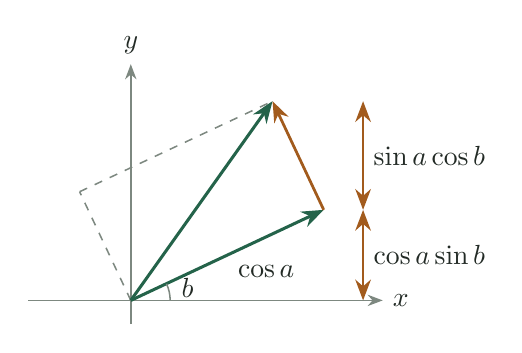
\begin{tikzpicture}[>=Stealth,font=\normalsize]
\draw[axis,->] (-1.3,0)--(3.2,0) node[right] {$x$};\draw[axis,->] (0,-.3)--(0,3) node[above] {$y$};
\coordinate(O) at(0,0);\coordinate(U) at(2.45,1.15);\coordinate(V) at(-.65,1.38);\coordinate(P) at(1.8,2.53);
\draw[main,->] (O)--(U) node[midway,below right] {$\cos a$};\draw[accent,->] (U)--(P);
\draw[axis,dashed] (O)--(V);\draw[axis,dashed] (V)--(P);\draw[main,->] (O)--(P);\draw[axis] (.5,0) arc(0:25:.5);\node at(.72,.16) {$b$};\draw[accent,<->] (2.95,0)--(2.95,1.15) node[midway,right] {$\cos a\sin b$};\draw[accent,<->] (2.95,1.15)--(2.95,2.53) node[midway,right] {$\sin a\cos b$};
\end{tikzpicture}

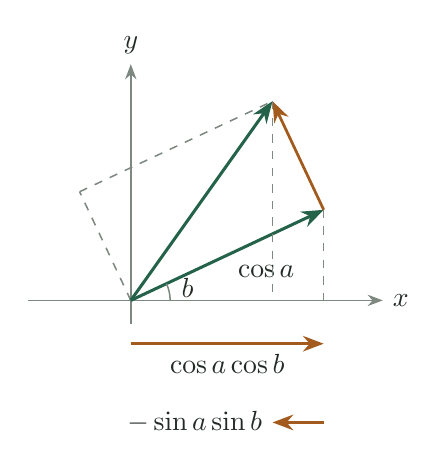
\begin{tikzpicture}[>=Stealth,font=\normalsize]
\draw[axis,->] (-1.3,0)--(3.2,0) node[right] {$x$};\draw[axis,->] (0,-.3)--(0,3) node[above] {$y$};
\coordinate(O) at(0,0);\coordinate(U) at(2.45,1.15);\coordinate(V) at(-.65,1.38);\coordinate(P) at(1.8,2.53);
\draw[main,->] (O)--(U) node[midway,below right] {$\cos a$};\draw[accent,->] (U)--(P);
\draw[axis,dashed] (O)--(V);\draw[axis,dashed] (V)--(P);\draw[main,->] (O)--(P);\draw[axis] (.5,0) arc(0:25:.5);\node at(.72,.16) {$b$};\draw[axis,dashed] (U)--(2.45,0);\draw[axis,dashed] (P)--(1.8,0);\draw[accent,->] (0,-.55)--(2.45,-.55) node[midway,below] {$\cos a\cos b$};\draw[accent,->] (2.45,-1.55)--(1.8,-1.55) node[left] {$-\sin a\sin b$};
\end{tikzpicture}

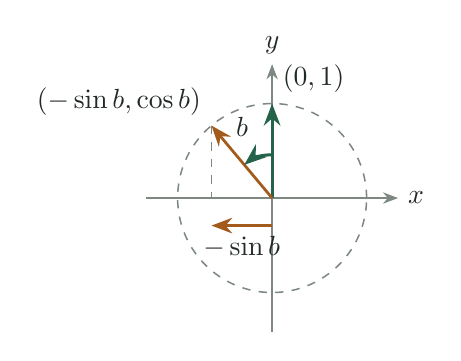
\begin{tikzpicture}[>=Stealth,font=\normalsize]
\draw[axis,->] (-1.6,0)--(1.6,0) node[right] {$x$};\draw[axis,->] (0,-1.7)--(0,1.7) node[above] {$y$};\draw[axis,dashed] (0,0) circle(1.2);\draw[main,->] (0,0)--(0,1.2) node[above right] {$(0,1)$};\draw[accent,->] (0,0)--(-.77,.92) node[above left] {$(-\sin b,\cos b)$};\draw[axis,dashed] (-.77,.92)--(-.77,0);\draw[accent,->] (0,-.35)--(-.77,-.35) node[midway,below] {$-\sin b$};\draw[main,->] (0,.55) arc(90:130:.55);\node at(-.38,.9) {$b$};
\end{tikzpicture}

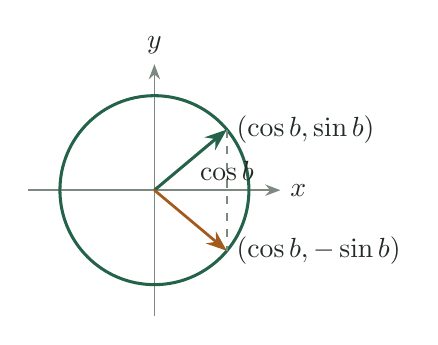
\begin{tikzpicture}[>=Stealth,font=\normalsize]
\draw[axis,->] (-1.6,0)--(1.6,0) node[right] {$x$};\draw[axis,->] (0,-1.6)--(0,1.6) node[above] {$y$};\draw[main] (0,0) circle(1.2);\draw[main,->] (0,0)--(.92,.77);\draw[accent,->] (0,0)--(.92,-.77);\draw[axis,dashed] (.92,.77)--(.92,-.77);\node[right] at(.92,.77) {$(\cos b,\sin b)$};\node[right] at(.92,-.77) {$(\cos b,-\sin b)$};\node[above] at(.92,0) {$\cos b$};
\end{tikzpicture}

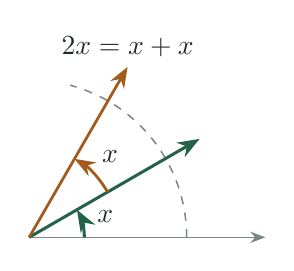
\begin{tikzpicture}[>=Stealth,font=\normalsize]
\draw[axis,->] (0,0)--(3,0);\draw[axis,dashed] (2,0) arc(0:75:2);\draw[main,->] (0,0)--(30:2.5);\draw[accent,->] (0,0)--(60:2.5);\draw[main,->] (.7,0) arc(0:30:.7);\draw[accent,->] (30:1.15) arc(30:60:1.15);\node at(15:1) {$x$};\node at(45:1.45) {$x$};\node[above] at(60:2.5) {$2x=x+x$};
\end{tikzpicture}

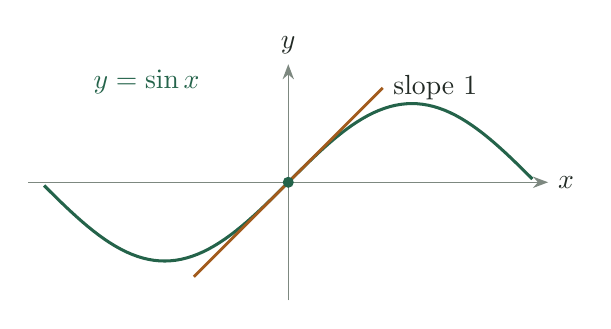
\begin{tikzpicture}[>=Stealth,font=\normalsize]
\draw[axis,->] (-3.3,0)--(3.3,0) node[right] {$x$};\draw[axis,->] (0,-1.5)--(0,1.5) node[above] {$y$};\draw[main,domain=-3.1:3.1,samples=90] plot(\x,{sin(\x r)});\draw[accent,domain=-1.2:1.2] plot(\x,\x) node[right] {slope $1$};\fill[ink] (0,0) circle(2pt);\node[ink,above] at (-1.8,1) {$y=\sin x$};
\end{tikzpicture}

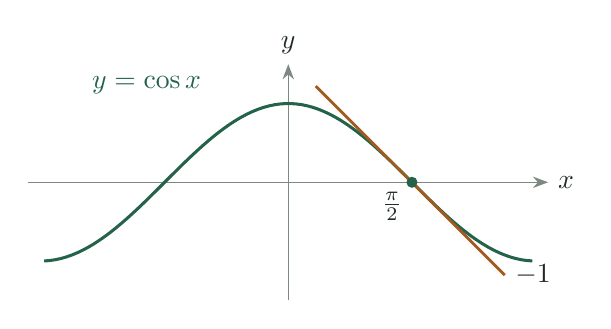
\begin{tikzpicture}[>=Stealth,font=\normalsize]
\draw[axis,->] (-3.3,0)--(3.3,0) node[right] {$x$};\draw[axis,->] (0,-1.5)--(0,1.5) node[above] {$y$};\draw[main,domain=-3.1:3.1,samples=90] plot(\x,{cos(\x r)});\draw[accent,domain=.35:2.75] plot(\x,{1.5708-\x}) node[right] {$-1$};\fill[ink] (1.5708,0) circle(2pt);\node[below left] at (1.57,0) {$\frac\pi2$};\node[ink,above] at (-1.8,1) {$y=\cos x$};
\end{tikzpicture}

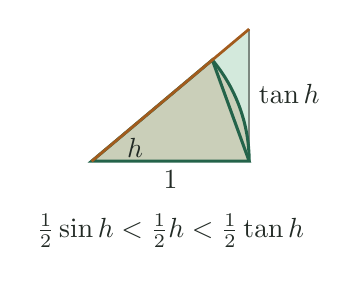
\begin{tikzpicture}[>=Stealth,font=\normalsize]
\coordinate(O) at(0,0);\coordinate(A) at(2,0);\coordinate(P) at(40:2);\coordinate(T) at(2,1.678);\fill[figurefill] (O)--(A)--(T)--cycle;\fill[accentink,opacity=.18] (O)--(A) arc(0:40:2)--cycle;\draw[axis] (A)--(T);\draw[main] (O)--(A)--(P)--cycle;\draw[main] (A) arc(0:40:2);\draw[accent] (O)--(T);\node[below] at(1,0) {$1$};\node at(.55,.17) {$h$};\node[right] at(2,.85) {$\tan h$};\node[below] at(1,-.55) {$\frac12\sin h<\frac12h<\frac12\tan h$};
\end{tikzpicture}

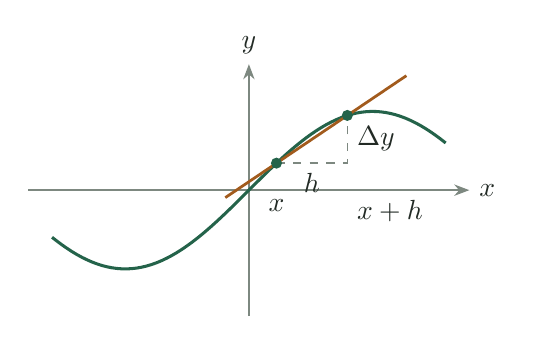
\begin{tikzpicture}[>=Stealth,font=\normalsize]
\draw[axis,->] (-2.8,0)--(2.8,0) node[right] {$x$};\draw[axis,->] (0,-1.6)--(0,1.6) node[above] {$y$};\draw[main,domain=-2.5:2.5,samples=80] plot(\x,{sin(\x r)});\coordinate(A) at(.35,.343);\coordinate(B) at(1.25,.949);\draw[accent] (-.3,-.095)--(2,1.454);\draw[axis,dashed] (A)--(1.25,.343)--(B);\fill[ink] (A) circle(2pt) (B) circle(2pt);\node[below] at(.8,.343) {$h$};\node[right] at(1.25,.65) {$\Delta y$};\node[below] at(.35,0) {$x$};\node[below right] at(1.25,0) {$x+h$};
\end{tikzpicture}

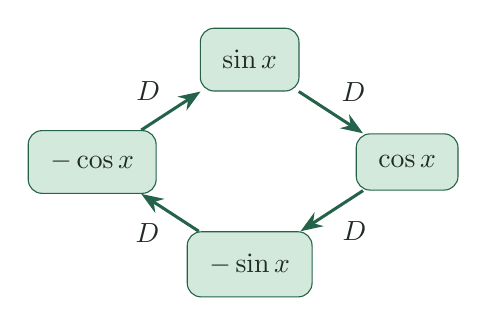
\begin{tikzpicture}[>=Stealth,font=\normalsize]
\node[box] (s) at(0,1.3) {$\sin x$};\node[box] (c) at(2,0) {$\cos x$};\node[box] (ns) at(0,-1.3) {$-\sin x$};\node[box] (nc) at(-2,0) {$-\cos x$};\draw[main,->] (s)--(c) node[midway,above right] {$D$};\draw[main,->] (c)--(ns) node[midway,below right] {$D$};\draw[main,->] (ns)--(nc) node[midway,below left] {$D$};\draw[main,->] (nc)--(s) node[midway,above left] {$D$};
\end{tikzpicture}

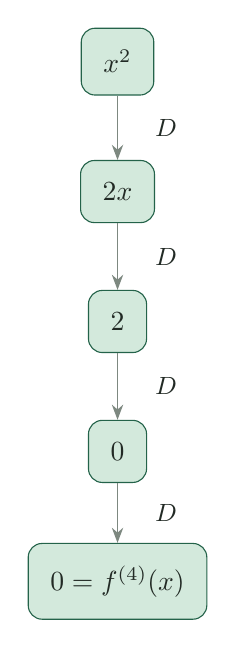
\begin{tikzpicture}[>=Stealth,font=\normalsize]
\node[box] (n0) at (0,-0.0) {$x^2$};\node[box] (n1) at (0,-1.65) {$2x$};\draw[->,axis] (n0)--(n1) node[midway,right=10pt,font=\small] {$D$};\node[box] (n2) at (0,-3.3) {$2$};\draw[->,axis] (n1)--(n2) node[midway,right=10pt,font=\small] {$D$};\node[box] (n3) at (0,-4.949999999999999) {$0$};\draw[->,axis] (n2)--(n3) node[midway,right=10pt,font=\small] {$D$};\node[box] (n4) at (0,-6.6) {$0=f^{(4)}(x)$};\draw[->,axis] (n3)--(n4) node[midway,right=10pt,font=\small] {$D$};
\end{tikzpicture}

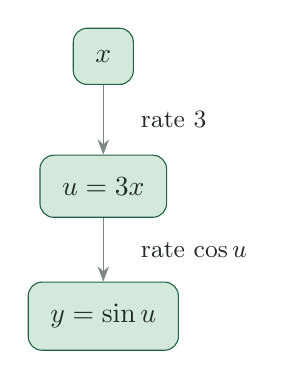
\begin{tikzpicture}[>=Stealth,font=\normalsize]
\node[box] (n0) at (0,-0.0) {$x$};\node[box] (n1) at (0,-1.65) {$u=3x$};\draw[->,axis] (n0)--(n1) node[midway,right=10pt,font=\small] {rate $3$};\node[box] (n2) at (0,-3.3) {$y=\sin u$};\draw[->,axis] (n1)--(n2) node[midway,right=10pt,font=\small] {rate $\cos u$};
\end{tikzpicture}

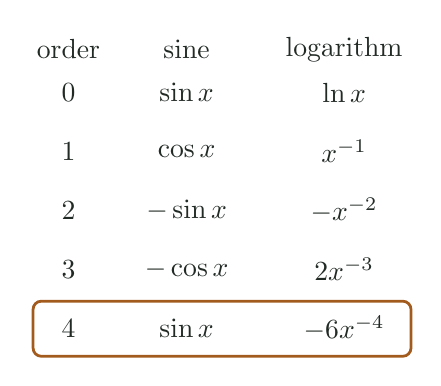
\begin{tikzpicture}[>=Stealth,font=\normalsize]
\node at(0,.55) {order};\node at(1.5,.55) {sine};\node at(3.5,.55) {logarithm};\foreach \n/\s/\l in {0/\sin x/\ln x,1/\cos x/x^{-1},2/-\sin x/-x^{-2},3/-\cos x/2x^{-3},4/\sin x/-6x^{-4}}{\node at(0,-.75*\n) {$\n$};\node at(1.5,-.75*\n) {$\s$};\node at(3.5,-.75*\n) {$\l$};}\draw[accent,rounded corners=3pt] (-.45,-3.35) rectangle(4.35,-2.65);
\end{tikzpicture}

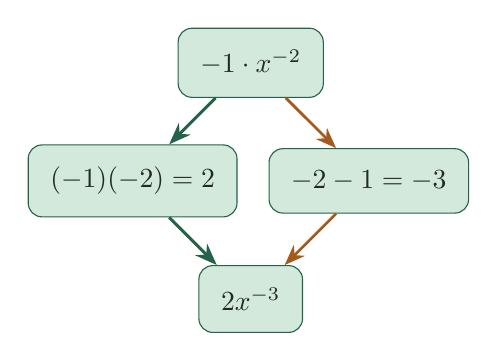
\begin{tikzpicture}[>=Stealth,font=\normalsize]
\node[box] (a) at(0,1) {$-1\cdot x^{-2}$};\node[box] (b) at(-1.5,-.5) {$(-1)(-2)=2$};\node[box] (c) at(1.5,-.5) {$-2-1=-3$};\draw[main,->] (a)--(b);\draw[accent,->] (a)--(c);\node[box] (d) at(0,-2) {$2x^{-3}$};\draw[main,->] (b)--(d);\draw[accent,->] (c)--(d);
\end{tikzpicture}

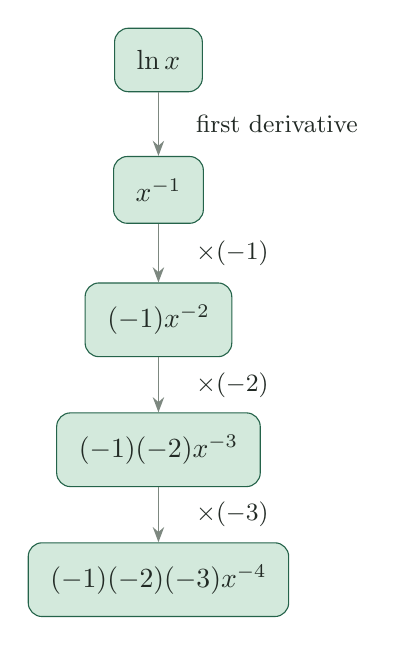
\begin{tikzpicture}[>=Stealth,font=\normalsize]
\node[box] (n0) at (0,-0.0) {$\ln x$};\node[box] (n1) at (0,-1.65) {$x^{-1}$};\draw[->,axis] (n0)--(n1) node[midway,right=10pt,font=\small] {first derivative};\node[box] (n2) at (0,-3.3) {$(-1)x^{-2}$};\draw[->,axis] (n1)--(n2) node[midway,right=10pt,font=\small] {$\times(-1)$};\node[box] (n3) at (0,-4.949999999999999) {$(-1)(-2)x^{-3}$};\draw[->,axis] (n2)--(n3) node[midway,right=10pt,font=\small] {$\times(-2)$};\node[box] (n4) at (0,-6.6) {$(-1)(-2)(-3)x^{-4}$};\draw[->,axis] (n3)--(n4) node[midway,right=10pt,font=\small] {$\times(-3)$};
\end{tikzpicture}

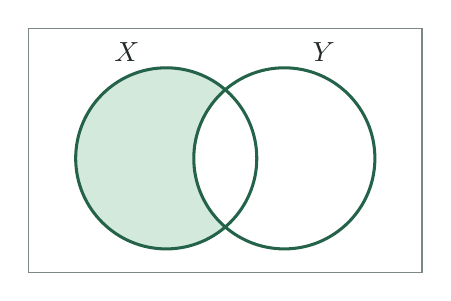
\begin{tikzpicture}[>=Stealth,font=\normalsize]
\draw[axis] (-2.5,-1.45) rectangle (2.5,1.65);\begin{scope}\clip (-.75,0) circle(1.15);\fill[figurefill,even odd rule] (-2.5,-1.5) rectangle(2.5,1.7) (.75,0) circle(1.15);\end{scope}\draw[main] (-.75,0) circle(1.15);\draw[main] (.75,0) circle(1.15);\node at (-1.25,1.35) {$X$};\node at (1.25,1.35) {$Y$};
\end{tikzpicture}

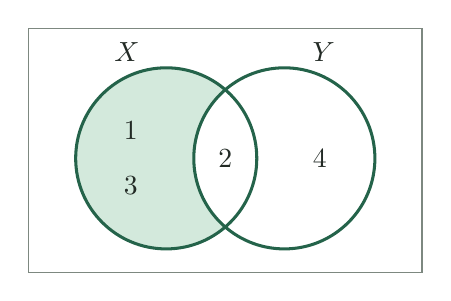
\begin{tikzpicture}[>=Stealth,font=\normalsize]
\draw[axis] (-2.5,-1.45) rectangle (2.5,1.65);\begin{scope}\clip (-.75,0) circle(1.15);\fill[figurefill,even odd rule] (-2.5,-1.5) rectangle(2.5,1.7) (.75,0) circle(1.15);\end{scope}\draw[main] (-.75,0) circle(1.15);\draw[main] (.75,0) circle(1.15);\node at (-1.25,1.35) {$X$};\node at (1.25,1.35) {$Y$};\node at (-1.2,.35) {$1$};\node at (-1.2,-.35) {$3$};\node at (0,0) {$2$};\node at (1.2,0) {$4$};
\end{tikzpicture}

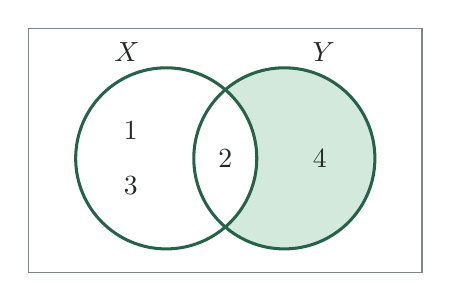
\begin{tikzpicture}[>=Stealth,font=\normalsize]
\draw[axis] (-2.5,-1.45) rectangle (2.5,1.65);\begin{scope}\clip (.75,0) circle(1.15);\fill[figurefill,even odd rule] (-2.5,-1.5) rectangle(2.5,1.7) (-.75,0) circle(1.15);\end{scope}\draw[main] (-.75,0) circle(1.15);\draw[main] (.75,0) circle(1.15);\node at (-1.25,1.35) {$X$};\node at (1.25,1.35) {$Y$};\node at (-1.2,.35) {$1$};\node at (-1.2,-.35) {$3$};\node at (0,0) {$2$};\node at (1.2,0) {$4$};
\end{tikzpicture}

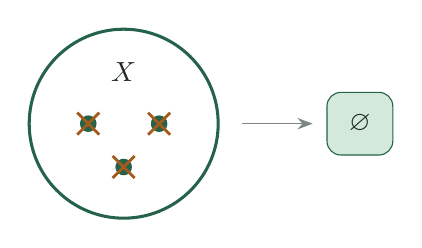
\begin{tikzpicture}[>=Stealth,font=\normalsize]
\draw[main] (0,0) circle(1.2);\node at(0,.65) {$X$};\foreach \x/\y in {-.45/0,.45/0,0/-.55}{\fill[ink] (\x,\y) circle(3pt);\draw[accent] (\x-.14,\y-.14)--(\x+.14,\y+.14);\draw[accent] (\x-.14,\y+.14)--(\x+.14,\y-.14);}\draw[axis,->] (1.5,0)--(2.4,0);\node[box] at(3,0) {$\varnothing$};
\end{tikzpicture}

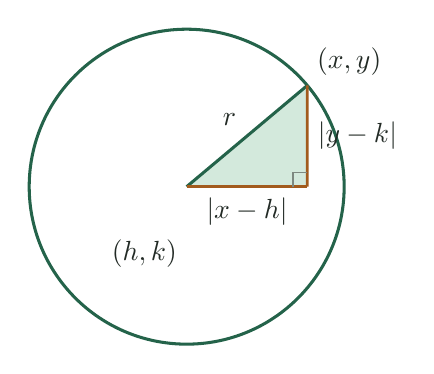
\begin{tikzpicture}[>=Stealth,font=\normalsize]
\draw[main] (0,0) circle(2);\coordinate(P) at(40:2);\fill[figurefill] (0,0)--(1.532,0)--(P)--cycle;\draw[main] (0,0)--(P) node[midway,above left] {$r$};\draw[accent] (0,0)--(1.532,0) node[midway,below] {$|x-h|$};\draw[accent] (1.532,0)--(P) node[midway,right] {$|y-k|$};\draw[axis] (1.35,0)--(1.35,.18)--(1.532,.18);\node[below left] at(0,-.55) {$(h,k)$};\node[above right] at(P) {$(x,y)$};
\end{tikzpicture}

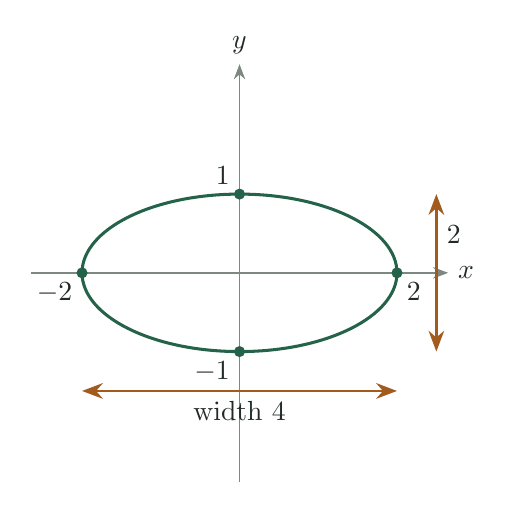
\begin{tikzpicture}[>=Stealth,font=\normalsize]
\draw[axis,->] (-2.65,0)--(2.65,0) node[right] {$x$};\draw[axis,->] (0,-2.65)--(0,2.65) node[above] {$y$};\draw[main] (0,0) ellipse (2.0 and 1.0);\fill[ink] (-2.0,0) circle(2pt) (2.0,0) circle(2pt) (0,-1.0) circle(2pt) (0,1.0) circle(2pt);\node[below left] at (-2.0,0) {$-2$};\node[below right] at (2.0,0) {$2$};\node[above left] at (0,1.0) {$1$};\node[below left] at (0,-1.0) {$-1$};\draw[accent,<->] (-2.0,-1.5)--(2.0,-1.5) node[midway,below] {width $4$};\draw[accent,<->] (2.5,-1.0)--(2.5,1.0) node[midway,right,yshift=14pt] {$2$};
\end{tikzpicture}

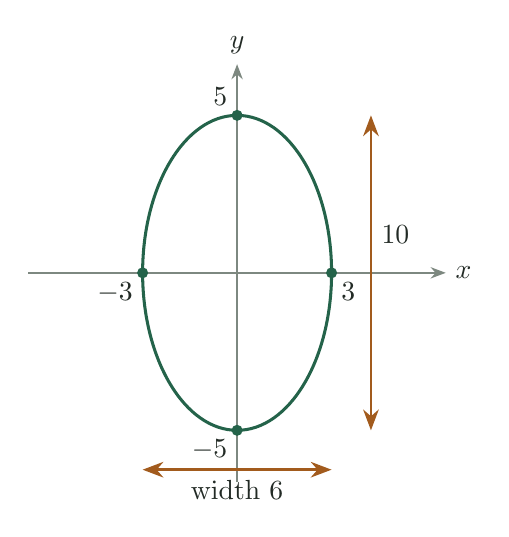
\begin{tikzpicture}[>=Stealth,font=\normalsize]
\draw[axis,->] (-2.65,0)--(2.65,0) node[right] {$x$};\draw[axis,->] (0,-2.65)--(0,2.65) node[above] {$y$};\draw[main] (0,0) ellipse (1.2000000000000002 and 2.0);\fill[ink] (-1.2000000000000002,0) circle(2pt) (1.2000000000000002,0) circle(2pt) (0,-2.0) circle(2pt) (0,2.0) circle(2pt);\node[below left] at (-1.2000000000000002,0) {$-3$};\node[below right] at (1.2000000000000002,0) {$3$};\node[above left] at (0,2.0) {$5$};\node[below left] at (0,-2.0) {$-5$};\draw[accent,<->] (-1.2000000000000002,-2.5)--(1.2000000000000002,-2.5) node[midway,below] {width $6$};\draw[accent,<->] (1.7000000000000002,-2.0)--(1.7000000000000002,2.0) node[midway,right,yshift=14pt] {$10$};
\end{tikzpicture}

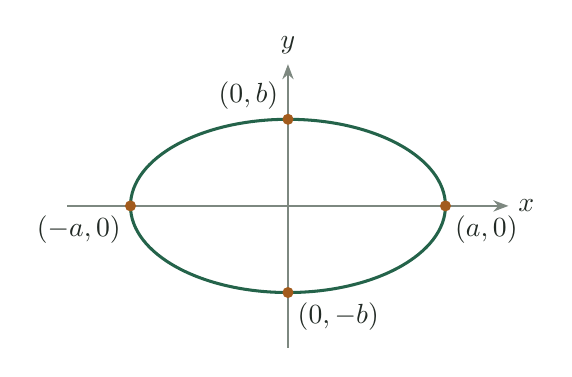
\begin{tikzpicture}[>=Stealth,font=\normalsize]
\draw[axis,->] (-2.8,0)--(2.8,0) node[right] {$x$};\draw[axis,->] (0,-1.8)--(0,1.8) node[above] {$y$};\draw[main] (0,0) ellipse(2 and 1.1);\fill[accentink] (-2,0) circle(2pt) (2,0) circle(2pt) (0,-1.1) circle(2pt) (0,1.1) circle(2pt);\node[below left] at(-2,0) {$(-a,0)$};\node[below right] at(2,0) {$(a,0)$};\node[above left] at(0,1.1) {$(0,b)$};\node[below right] at(0,-1.1) {$(0,-b)$};
\end{tikzpicture}

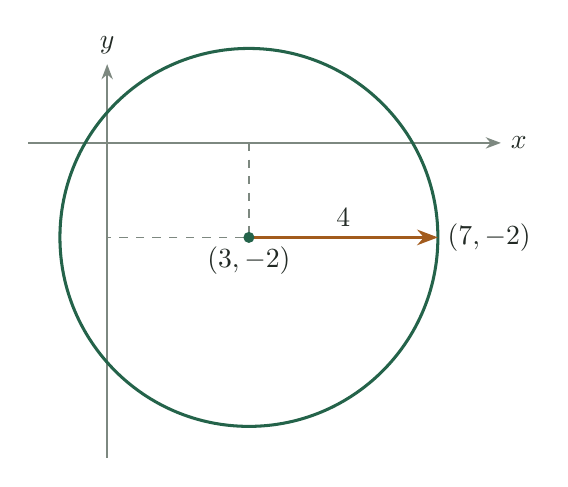
\begin{tikzpicture}[>=Stealth,font=\normalsize]
\draw[axis,->] (-1,0)--(5,0) node[right] {$x$};\draw[axis,->] (0,-4)--(0,1) node[above] {$y$};\draw[main] (1.8,-1.2) circle(2.4);\draw[axis,dashed] (1.8,0)--(1.8,-1.2)--(0,-1.2);\draw[accent,->] (1.8,-1.2)--(4.2,-1.2) node[midway,above] {$4$};\fill[ink] (1.8,-1.2) circle(2pt);\node[below] at(1.8,-1.2) {$(3,-2)$};\node[right] at(4.2,-1.2) {$(7,-2)$};
\end{tikzpicture}

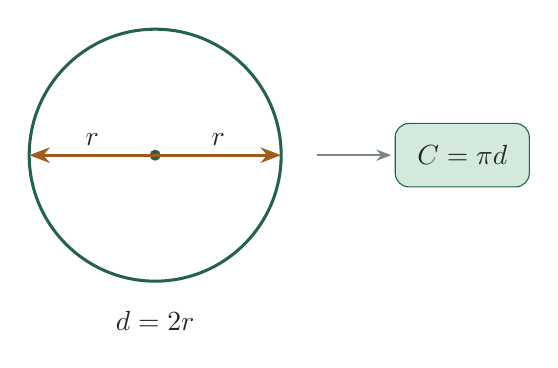
\begin{tikzpicture}[>=Stealth,font=\normalsize]
\draw[main] (0,0) circle(1.6);\fill[ink] (0,0) circle(2pt);\draw[accent,<->] (-1.6,0)--(1.6,0);\node[above] at(-.8,0) {$r$};\node[above] at(.8,0) {$r$};\node at(0,-2.1) {$d=2r$};\draw[axis,->] (2.05,0)--(3,0);\node[box] at(3.9,0) {$C=\pi d$};
\end{tikzpicture}

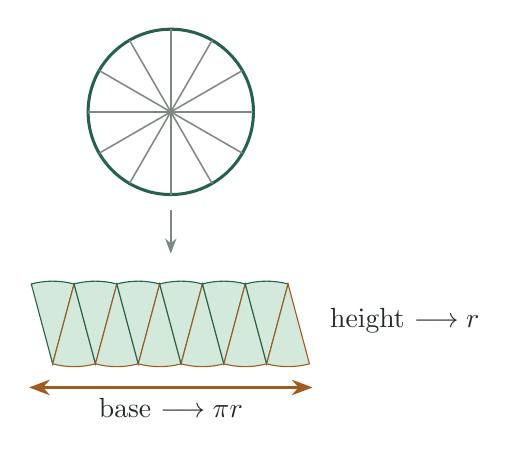
\begin{tikzpicture}[>=Stealth,font=\normalsize]
\draw[main] (0,2.65) circle(1.05);\foreach \a in {0,30,...,330}{\draw[axis] (0,2.65)--++(\a:1.05);}\draw[axis,->] (0,1.4)--(0,.85);\begin{scope}[shift={(-1.5,-.55)}]\filldraw[fill=figurefill,draw=ink] (0,0)--(75:1.05) arc(75:105:1.05)--cycle;\end{scope}\begin{scope}[shift={(-1.22824,.46422)}]\filldraw[fill=figurefill,draw=accentink] (0,0)--(255:1.05) arc(255:285:1.05)--cycle;\end{scope}\begin{scope}[shift={(-0.95648,-.55)}]\filldraw[fill=figurefill,draw=ink] (0,0)--(75:1.05) arc(75:105:1.05)--cycle;\end{scope}\begin{scope}[shift={(-0.68472,.46422)}]\filldraw[fill=figurefill,draw=accentink] (0,0)--(255:1.05) arc(255:285:1.05)--cycle;\end{scope}\begin{scope}[shift={(-0.41296,-.55)}]\filldraw[fill=figurefill,draw=ink] (0,0)--(75:1.05) arc(75:105:1.05)--cycle;\end{scope}\begin{scope}[shift={(-0.1412,.46422)}]\filldraw[fill=figurefill,draw=accentink] (0,0)--(255:1.05) arc(255:285:1.05)--cycle;\end{scope}\begin{scope}[shift={(0.13056,-.55)}]\filldraw[fill=figurefill,draw=ink] (0,0)--(75:1.05) arc(75:105:1.05)--cycle;\end{scope}\begin{scope}[shift={(0.40232,.46422)}]\filldraw[fill=figurefill,draw=accentink] (0,0)--(255:1.05) arc(255:285:1.05)--cycle;\end{scope}\begin{scope}[shift={(0.67408,-.55)}]\filldraw[fill=figurefill,draw=ink] (0,0)--(75:1.05) arc(75:105:1.05)--cycle;\end{scope}\begin{scope}[shift={(0.94584,.46422)}]\filldraw[fill=figurefill,draw=accentink] (0,0)--(255:1.05) arc(255:285:1.05)--cycle;\end{scope}\begin{scope}[shift={(1.2176,-.55)}]\filldraw[fill=figurefill,draw=ink] (0,0)--(75:1.05) arc(75:105:1.05)--cycle;\end{scope}\begin{scope}[shift={(1.48936,.46422)}]\filldraw[fill=figurefill,draw=accentink] (0,0)--(255:1.05) arc(255:285:1.05)--cycle;\end{scope}\draw[accent,<->] (-1.8,-.85)--(1.8,-.85) node[midway,below] {base $\longrightarrow\pi r$};\node[right] at(1.9,0) {height $\longrightarrow r$};
\end{tikzpicture}

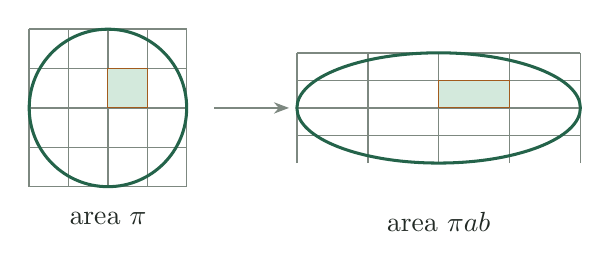
\begin{tikzpicture}[>=Stealth,font=\normalsize]
\begin{scope}[shift={(-2,0)}]\draw[axis,step=.5] (-1,-1) grid(1,1);\draw[main] (0,0) circle(1);\filldraw[fill=figurefill,draw=accentink] (0,0) rectangle(.5,.5);\node[below] at(0,-1.2) {area $\pi$};\end{scope}\draw[axis,->] (-.65,0)--(.3,0);\begin{scope}[shift={(2.2,0)}]\draw[axis,xstep=.9,ystep=.35] (-1.8,-.7) grid(1.8,.7);\draw[main] (0,0) ellipse(1.8 and .7);\filldraw[fill=figurefill,draw=accentink] (0,0) rectangle(.9,.35);\node[below] at(0,-1.2) {area $\pi ab$};\end{scope}
\end{tikzpicture}

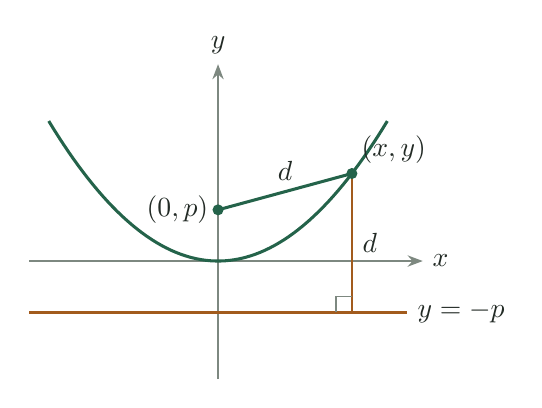
\begin{tikzpicture}[>=Stealth,font=\normalsize]
\draw[axis,->] (-2.4,0)--(2.6,0) node[right] {$x$};\draw[axis,->] (0,-1.5)--(0,2.5) node[above] {$y$};\draw[accent] (-2.4,-.65)--(2.4,-.65) node[right] {$y=-p$};\draw[main,domain=-2.15:2.15,samples=70] plot(\x,{\x*\x/2.6});\coordinate(P) at(1.7,1.1115);\fill[ink] (0,.65) circle(2pt) node[left] {$(0,p)$};\draw[main] (0,.65)--(P) node[midway,above] {$d$};\draw[accent] (P)--(1.7,-.65) node[midway,right] {$d$};\fill[ink] (P) circle(2pt) node[above right] {$(x,y)$};\draw[axis] (1.5,-.65)--(1.5,-.45)--(1.7,-.45);
\end{tikzpicture}

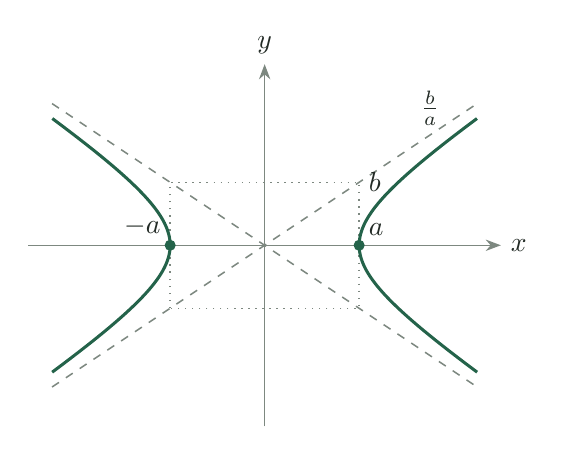
\begin{tikzpicture}[>=Stealth,font=\normalsize]
\draw[axis,->] (-3,0)--(3,0) node[right] {$x$};\draw[axis,->] (0,-2.3)--(0,2.3) node[above] {$y$};\draw[axis,dashed] (-2.7,-1.8)--(2.7,1.8);\draw[axis,dashed] (-2.7,1.8)--(2.7,-1.8);\draw[axis,dotted] (-1.2,-.8) rectangle(1.2,.8);\foreach \sgn in {-1,1}{\draw[main,domain=-1.45:1.45,samples=80] plot({\sgn*1.2*cosh(\x)},{.8*sinh(\x)});}\fill[ink] (-1.2,0) circle(2pt) (1.2,0) circle(2pt);\node[above left] at(-1.2,0) {$-a$};\node[above right] at(1.2,0) {$a$};\node[right] at(1.2,.8) {$b$};\node[above] at(2.1,1.4) {$\frac ba$};
\end{tikzpicture}

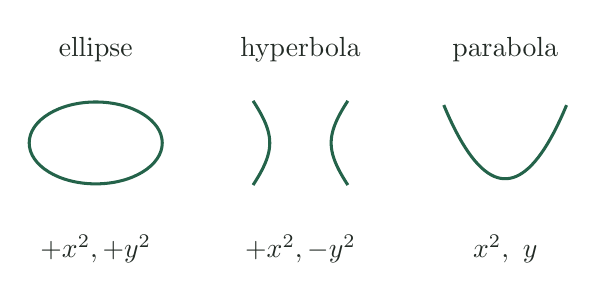
\begin{tikzpicture}[>=Stealth,font=\normalsize]
\begin{scope}[shift={(-2.6,0)},scale=.65]\draw[main] (0,0) ellipse(1.3 and .8);\node[below] at(0,-1.6) {$+x^2,+y^2$};\node[above] at(0,1.4) {ellipse};\end{scope}\begin{scope}[scale=.65]\foreach \s in {-1,1}{\draw[main,domain=-1:1,samples=40] plot({\s*.6*cosh(\x)},{.7*sinh(\x)});}\node[below] at(0,-1.6) {$+x^2,-y^2$};\node[above] at(0,1.4) {hyperbola};\end{scope}\begin{scope}[shift={(2.6,0)},scale=.65]\draw[main,domain=-1.2:1.2,samples=40] plot(\x,{\x*\x-.7});\node[below] at(0,-1.6) {$x^2,\ y$};\node[above] at(0,1.4) {parabola};\end{scope}
\end{tikzpicture}

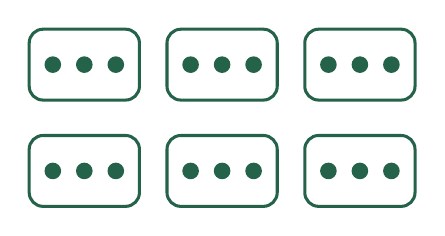
\begin{tikzpicture}[>=Stealth,font=\normalsize]
\draw[main,rounded corners=5pt] (-0.45,-0.45) rectangle(0.95,0.45);\fill[ink] (-0.15,0.0) circle(3pt);\fill[ink] (0.25,0.0) circle(3pt);\fill[ink] (0.65,0.0) circle(3pt);\draw[main,rounded corners=5pt] (1.3,-0.45) rectangle(2.7,0.45);\fill[ink] (1.6,0.0) circle(3pt);\fill[ink] (2.0,0.0) circle(3pt);\fill[ink] (2.4,0.0) circle(3pt);\draw[main,rounded corners=5pt] (3.05,-0.45) rectangle(4.45,0.45);\fill[ink] (3.35,0.0) circle(3pt);\fill[ink] (3.75,0.0) circle(3pt);\fill[ink] (4.1499999999999995,0.0) circle(3pt);\draw[main,rounded corners=5pt] (-0.45,-1.8) rectangle(0.95,-0.9000000000000001);\fill[ink] (-0.15,-1.35) circle(3pt);\fill[ink] (0.25,-1.35) circle(3pt);\fill[ink] (0.65,-1.35) circle(3pt);\draw[main,rounded corners=5pt] (1.3,-1.8) rectangle(2.7,-0.9000000000000001);\fill[ink] (1.6,-1.35) circle(3pt);\fill[ink] (2.0,-1.35) circle(3pt);\fill[ink] (2.4,-1.35) circle(3pt);\draw[main,rounded corners=5pt] (3.05,-1.8) rectangle(4.45,-0.9000000000000001);\fill[ink] (3.35,-1.35) circle(3pt);\fill[ink] (3.75,-1.35) circle(3pt);\fill[ink] (4.1499999999999995,-1.35) circle(3pt);
\end{tikzpicture}

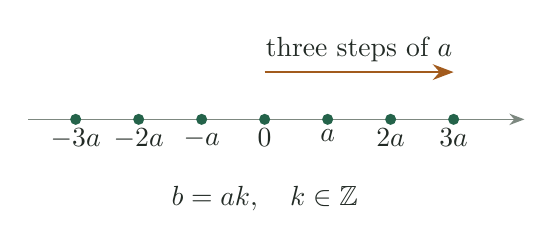
\begin{tikzpicture}[>=Stealth,font=\normalsize]
\draw[axis,->] (-3,0)--(3.3,0);\foreach \x/\lab in {-2.4/-3a,-1.6/-2a,-.8/-a,0/0,.8/a,1.6/2a,2.4/3a}{\fill[ink] (\x,0) circle(2pt);\node[below] at(\x,0) {$\lab$};}\draw[accent,->] (0,.6)--(2.4,.6) node[midway,above] {three steps of $a$};\node at(0,-1) {$b=ak,\quad k\in\mathbb Z$};
\end{tikzpicture}

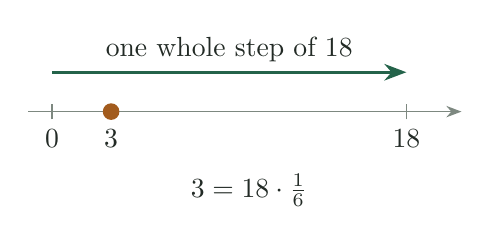
\begin{tikzpicture}[>=Stealth,font=\normalsize]
\draw[axis,->] (-.3,0)--(5.2,0);\foreach \x/\lab in {0/0,.75/3,4.5/18}{\draw[axis] (\x,-.1)--(\x,.1);\node[below] at(\x,-.1) {$\lab$};}\draw[main,->] (0,.5)--(4.5,.5) node[midway,above] {one whole step of $18$};\fill[accentink] (.75,0) circle(3pt);\node at(2.5,-1) {$3=18\cdot\frac16$};
\end{tikzpicture}

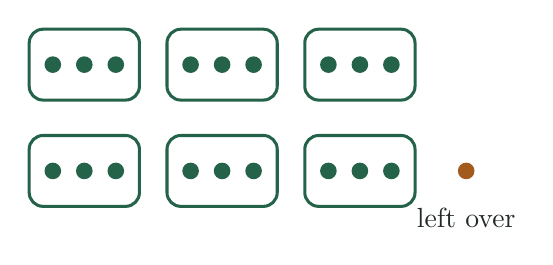
\begin{tikzpicture}[>=Stealth,font=\normalsize]
\draw[main,rounded corners=5pt] (-0.45,-0.45) rectangle(0.95,0.45);\fill[ink] (-0.15,0.0) circle(3pt);\fill[ink] (0.25,0.0) circle(3pt);\fill[ink] (0.65,0.0) circle(3pt);\draw[main,rounded corners=5pt] (1.3,-0.45) rectangle(2.7,0.45);\fill[ink] (1.6,0.0) circle(3pt);\fill[ink] (2.0,0.0) circle(3pt);\fill[ink] (2.4,0.0) circle(3pt);\draw[main,rounded corners=5pt] (3.05,-0.45) rectangle(4.45,0.45);\fill[ink] (3.35,0.0) circle(3pt);\fill[ink] (3.75,0.0) circle(3pt);\fill[ink] (4.1499999999999995,0.0) circle(3pt);\draw[main,rounded corners=5pt] (-0.45,-1.8) rectangle(0.95,-0.9000000000000001);\fill[ink] (-0.15,-1.35) circle(3pt);\fill[ink] (0.25,-1.35) circle(3pt);\fill[ink] (0.65,-1.35) circle(3pt);\draw[main,rounded corners=5pt] (1.3,-1.8) rectangle(2.7,-0.9000000000000001);\fill[ink] (1.6,-1.35) circle(3pt);\fill[ink] (2.0,-1.35) circle(3pt);\fill[ink] (2.4,-1.35) circle(3pt);\draw[main,rounded corners=5pt] (3.05,-1.8) rectangle(4.45,-0.9000000000000001);\fill[ink] (3.35,-1.35) circle(3pt);\fill[ink] (3.75,-1.35) circle(3pt);\fill[ink] (4.1499999999999995,-1.35) circle(3pt);\fill[accentink] (5.1,-1.35) circle(3pt);\node[below] at (5.1,-1.7) {left over};
\end{tikzpicture}

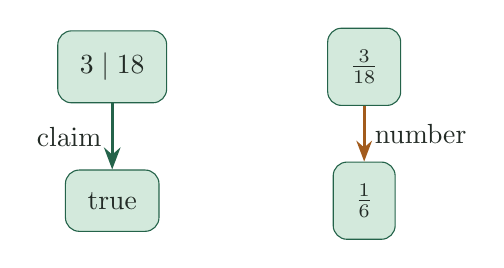
\begin{tikzpicture}[>=Stealth,font=\normalsize]
\node[box] (a) at(-1.6,1) {$3\mid18$};\node[box] (b) at(1.6,1) {$\frac3{18}$};\node[box] (c) at(-1.6,-.7) {true};\node[box] (d) at(1.6,-.7) {$\frac16$};\draw[main,->] (a)--(c) node[midway,left] {claim};\draw[accent,->] (b)--(d) node[midway,right] {number};
\end{tikzpicture}

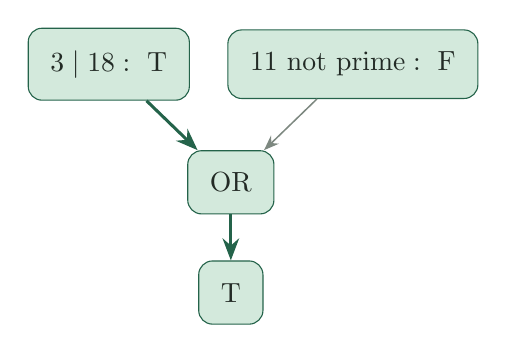
\begin{tikzpicture}[>=Stealth,font=\normalsize]
\node[box] (p) at(-1.55,1) {$3\mid18:\ \mathrm{T}$};\node[box] (q) at(1.55,1) {$11\text{ not prime}:\ \mathrm{F}$};\node[box] (o) at(0,-.5) {$\mathrm{OR}$};\draw[main,->] (p)--(o);\draw[axis,->] (q)--(o);\node[box] (t) at(0,-1.9) {$\mathrm{T}$};\draw[main,->] (o)--(t);
\end{tikzpicture}

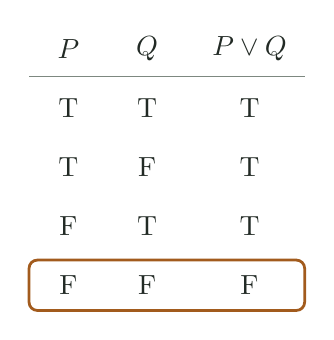
\begin{tikzpicture}[>=Stealth,font=\normalsize]
\node at(-1,1.3) {$P$};\node at(0,1.3) {$Q$};\node at(1.3,1.3) {$P\lor Q$};\draw[axis] (-1.5,.95)--(2,.95);\foreach \y/\p/\q/\r in {.55/T/T/T,-.2/T/F/T,-.95/F/T/T,-1.7/F/F/F}{\node at(-1,\y) {$\mathrm{\p}$};\node at(0,\y) {$\mathrm{\q}$};\node at(1.3,\y) {$\mathrm{\r}$};}\draw[accent,rounded corners=3pt] (-1.5,-2.02) rectangle(2,-1.38);
\end{tikzpicture}

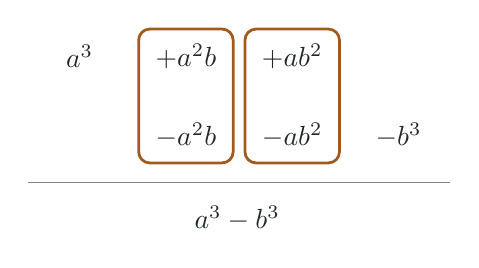
\begin{tikzpicture}[>=Stealth,font=\normalsize]
\node at(0.0,.5) {$a^3$};\node at(1.35,.5) {$+a^2b$};\node at(2.7,.5) {$+ab^2$};\node at(4.050000000000001,.5) {$$};\node at(0.0,-.5) {$$};\node at(1.35,-.5) {$-a^2b$};\node at(2.7,-.5) {$-ab^2$};\node at(4.050000000000001,-.5) {$-b^3$};\draw[axis] (-.65,-1.1)--(4.7,-1.1);\draw[accent,rounded corners=4pt] (0.7500000000000001,-.85) rectangle(1.9500000000000002,.85);\draw[accent,rounded corners=4pt] (2.1,-.85) rectangle(3.3000000000000003,.85);\node at(2,-1.55) {$a^3-b^3$};
\end{tikzpicture}

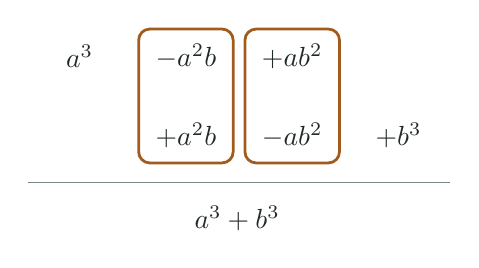
\begin{tikzpicture}[>=Stealth,font=\normalsize]
\node at(0.0,.5) {$a^3$};\node at(1.35,.5) {$-a^2b$};\node at(2.7,.5) {$+ab^2$};\node at(4.050000000000001,.5) {$$};\node at(0.0,-.5) {$$};\node at(1.35,-.5) {$+a^2b$};\node at(2.7,-.5) {$-ab^2$};\node at(4.050000000000001,-.5) {$+b^3$};\draw[axis] (-.65,-1.1)--(4.7,-1.1);\draw[accent,rounded corners=4pt] (0.7500000000000001,-.85) rectangle(1.9500000000000002,.85);\draw[accent,rounded corners=4pt] (2.1,-.85) rectangle(3.3000000000000003,.85);\node at(2,-1.55) {$a^3+b^3$};
\end{tikzpicture}

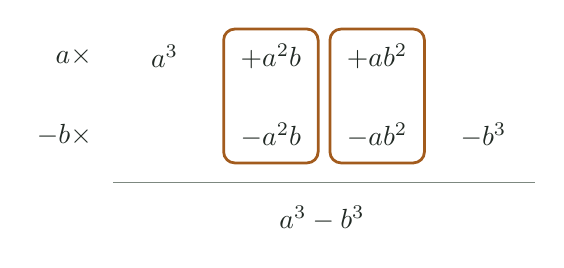
\begin{tikzpicture}[>=Stealth,font=\normalsize]
\node at(0.0,.5) {$a^3$};\node at(1.35,.5) {$+a^2b$};\node at(2.7,.5) {$+ab^2$};\node at(4.050000000000001,.5) {$$};\node at(0.0,-.5) {$$};\node at(1.35,-.5) {$-a^2b$};\node at(2.7,-.5) {$-ab^2$};\node at(4.050000000000001,-.5) {$-b^3$};\draw[axis] (-.65,-1.1)--(4.7,-1.1);\draw[accent,rounded corners=4pt] (0.7500000000000001,-.85) rectangle(1.9500000000000002,.85);\draw[accent,rounded corners=4pt] (2.1,-.85) rectangle(3.3000000000000003,.85);\node at(2,-1.55) {$a^3-b^3$};\node[left] at(-.8,.5) {$a\times$};\node[left] at(-.8,-.5) {$-b\times$};
\end{tikzpicture}

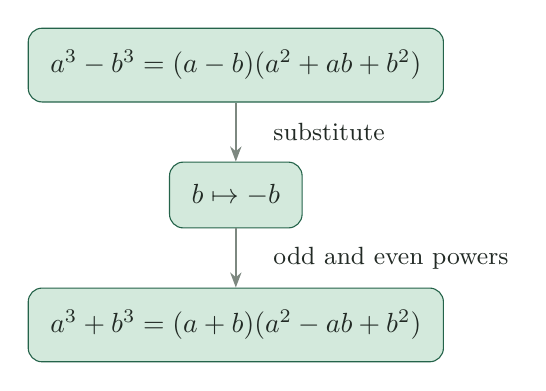
\begin{tikzpicture}[>=Stealth,font=\normalsize]
\node[box] (n0) at (0,-0.0) {$a^3-b^3=(a-b)(a^2+ab+b^2)$};\node[box] (n1) at (0,-1.65) {$b\mapsto-b$};\draw[->,axis] (n0)--(n1) node[midway,right=10pt,font=\small] {substitute};\node[box] (n2) at (0,-3.3) {$a^3+b^3=(a+b)(a^2-ab+b^2)$};\draw[->,axis] (n1)--(n2) node[midway,right=10pt,font=\small] {odd and even powers};
\end{tikzpicture}

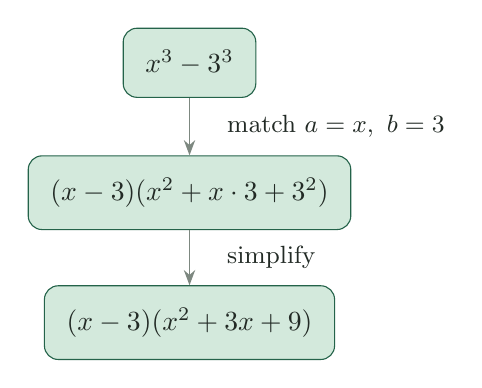
\begin{tikzpicture}[>=Stealth,font=\normalsize]
\node[box] (n0) at (0,-0.0) {$x^3-3^3$};\node[box] (n1) at (0,-1.65) {$(x-3)(x^2+x\cdot3+3^2)$};\draw[->,axis] (n0)--(n1) node[midway,right=10pt,font=\small] {match $a=x,\ b=3$};\node[box] (n2) at (0,-3.3) {$(x-3)(x^2+3x+9)$};\draw[->,axis] (n1)--(n2) node[midway,right=10pt,font=\small] {simplify};
\end{tikzpicture}

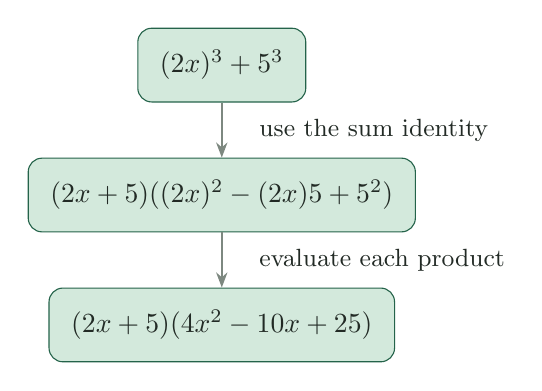
\begin{tikzpicture}[>=Stealth,font=\normalsize]
\node[box] (n0) at (0,-0.0) {$(2x)^3+5^3$};\node[box] (n1) at (0,-1.65) {$(2x+5)((2x)^2-(2x)5+5^2)$};\draw[->,axis] (n0)--(n1) node[midway,right=10pt,font=\small] {use the sum identity};\node[box] (n2) at (0,-3.3) {$(2x+5)(4x^2-10x+25)$};\draw[->,axis] (n1)--(n2) node[midway,right=10pt,font=\small] {evaluate each product};
\end{tikzpicture}

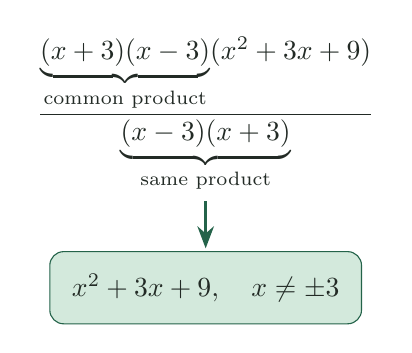
\begin{tikzpicture}[>=Stealth,font=\normalsize]
\node at(0,1) {$\displaystyle\frac{\underbrace{(x+3)(x-3)}_{\text{common product}}(x^2+3x+9)}{\underbrace{(x-3)(x+3)}_{\text{same product}}}$};\draw[main,->] (0,-.1)--(0,-.7);\node[box] at(0,-1.2) {$x^2+3x+9,\quad x\ne\pm3$};
\end{tikzpicture}

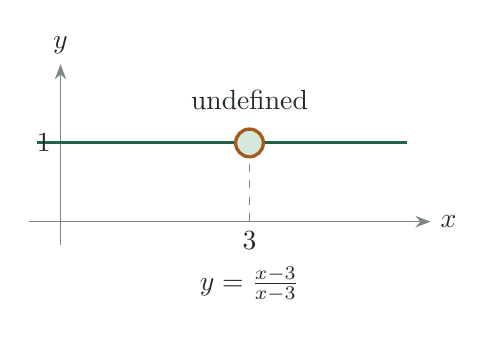
\begin{tikzpicture}[>=Stealth,font=\normalsize]
\draw[axis,->] (-.4,0)--(4.7,0) node[right] {$x$};\draw[axis,->] (0,-.3)--(0,2) node[above] {$y$};\draw[main] (-.3,1)--(4.4,1);\fill[figurefill] (2.4,1) circle(5pt);\draw[accent,very thick] (2.4,1) circle(5pt);\draw[axis,dashed] (2.4,0)--(2.4,.85);\node[below] at(2.4,0) {$3$};\node[left] at(0,1) {$1$};\node[above] at(2.4,1.3) {undefined};\node at(2.4,-.8) {$y=\frac{x-3}{x-3}$};
\end{tikzpicture}

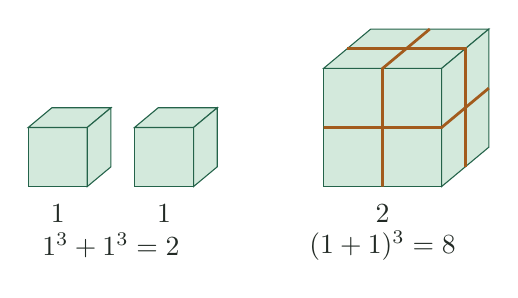
\begin{tikzpicture}[>=Stealth,font=\normalsize]
\begin{scope}[x={(.75cm,0cm)},y={(.3cm,.25cm)},z={(0cm,.75cm)}]\filldraw[fill=figurefill,draw=ink] (0,0,0)--(1,0,0)--(1,0,1)--(0,0,1)--cycle;\filldraw[fill=figurefill,draw=ink] (0,0,1)--(1,0,1)--(1,1,1)--(0,1,1)--cycle;\filldraw[fill=figurefill,draw=ink] (1,0,0)--(1,1,0)--(1,1,1)--(1,0,1)--cycle;\filldraw[fill=figurefill,draw=ink] (1.8,0,0)--(2.8,0,0)--(2.8,0,1)--(1.8,0,1)--cycle;\filldraw[fill=figurefill,draw=ink] (1.8,0,1)--(2.8,0,1)--(2.8,1,1)--(1.8,1,1)--cycle;\filldraw[fill=figurefill,draw=ink] (2.8,0,0)--(2.8,1,0)--(2.8,1,1)--(2.8,0,1)--cycle;\node at(.5,0,-.45) {$1$};\node at(2.3,0,-.45) {$1$};\node at(1.4,0,-1) {$1^3+1^3=2$};\filldraw[fill=figurefill,draw=ink] (5,0,0)--(7,0,0)--(7,0,2)--(5,0,2)--cycle;\filldraw[fill=figurefill,draw=ink] (5,0,2)--(7,0,2)--(7,2,2)--(5,2,2)--cycle;\filldraw[fill=figurefill,draw=ink] (7,0,0)--(7,2,0)--(7,2,2)--(7,0,2)--cycle;\draw[accent] (6,0,0)--(6,0,2)--(6,2,2);\draw[accent] (5,0,1)--(7,0,1)--(7,2,1);\draw[accent] (5,1,2)--(7,1,2)--(7,1,0);\node at(6,0,-.45) {$2$};\node at(6,0,-1) {$(1+1)^3=8$};\end{scope}
\end{tikzpicture}

\end{document}
